\documentclass[12 pt]{article}
\hbadness=10


\usepackage{amsmath, amssymb, amsfonts, setspace, stmaryrd, amsthm, graphicx, tikz}
\usepackage[utf8]{inputenc}
\usepackage[english]{babel}
\usetikzlibrary{positioning}% To get more advances positioning options
\usetikzlibrary{arrows}% To get more arrow heads
\usepackage{hyperref} % Allows to make references and links clickable

\usepackage[margin=1.5in]{geometry}
\newtheorem{theorem}{Theorem}
\newtheorem{definition}{Definition}
%%align* environment
\newcommand{\eq}[1]{\begin{align*}#1\end{align*}}

%Math commands
\DeclareMathOperator{\R}{\mathbb{R}}
\DeclareMathOperator{\C}{\mathbb{C}}
\DeclareMathOperator{\Z}{\mathbb{Z}}
\DeclareMathOperator{\N}{\mathbb{N}}
\DeclareMathOperator{\Q}{\mathbb{Q}}

\renewcommand\abstractname{Introduction}

\newcounter{exercise}[section]
\newenvironment{exercise}{\refstepcounter{exercise}\par\bigskip \begin{quotation}{}{\leftmargin .25in\rightmargin .25in}
	\noindent \textbf{Exercise~\thesection.\theexercise }  \rmfamily}{\end{quotation}\par\bigskip}
	

\newenvironment{bonus}{\refstepcounter{exercise}\par\bigskip \begin{quotation}{}{\leftmargin .25in\rightmargin .25in}
	\noindent \textbf{*Bonus Exercise*~\thesection.\theexercise }  \rmfamily}{\end{quotation}\par\bigskip}
	 


\title{Knot Theory}
\author{Girls Talk Math}
\date{}

\begin{document}
\maketitle
\vskip 1in
\begin{center} \textbf{Introduction} \end{center}
The mathematical study of knots is a large area of active mathematical research. Knot theory has applications in many distinct areas of mathematics, including algebra and geometry, as well as areas outside of mathematics, like physics. In this document, we will get a handle on what a knot is, learn how to describe it mathematically, and get an idea of some of the problems that knot theory was developed to answer. We will learn how to describe knots with some algebraic techniques, examine some features of the knots which these convey, and learn some other interesting algebraic properties of knots.

One last note about reading mathematical texts: it is very normal when reading math to read a passage or even a single sentence several times before understanding it properly. Also, never trust the author! Check every claim and calculation (time permitting). Take your time and never give up. Let's talk math!
	
\newpage

\tableofcontents

%%%%%%%%%%%%%%%%%%%%%%
%%% Use \section{}, \subsection{}, etc. for different parts of the problem set. Start a newpage for a new section
%%%%%%%%%%%%%%%%%%%%%%

%%%%%%%%%%%%%%%%%%%%%%%%%%%%%%%%%
%%%
%%% Embed exercises in section as appropriate 
%%% 
%%%%%%%%%%%%%%%%%%%%%%%%%%%%%%%%%%%

\newpage
\section{What are Knots and Links?}

First, we need to define some key concepts. A \textbf{knot} $\mathcal{K}$ is simply a loop in 3-dimensional space (that doesn't intersect itself). In practice, one thinks of tying a string into a knot and then connecting the two ends of the string (we'll later see why it's useful to connect the two ends of the string). The most basic knot there is the \textbf{unknot}, which is just a circle. One can also take a figure-eight, or square knot, etc., and connect the free ends of string to get a knot (as described before). A \textbf{link} is just several knots which don't intersect each other. For example, two interlocking circles that can't be pulled apart form a link consisting of two unknots. Here are two examples, the first of a knot, the second of a link:
\begin{center}
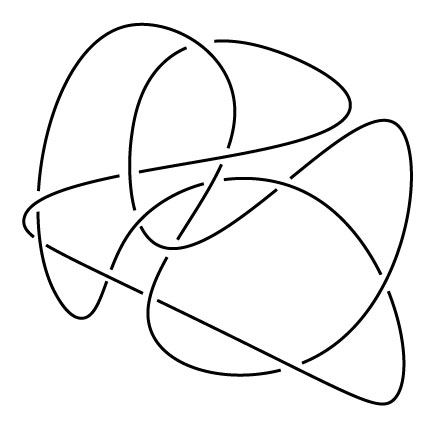
\includegraphics[height = 2in]{knot_ex_1.jpg} \quad 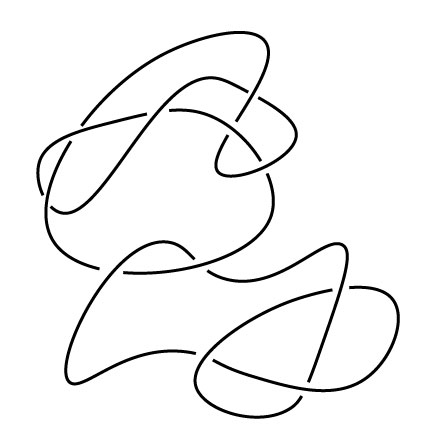
\includegraphics[height = 2in]{knot_ex_2.jpg}
\end{center}

Every time we introduce a new concept in math, we also should describe what it means for two things to be the same. For example, the numbers $1/2$ and $3/6$ are the same even though they look different. We say that two knots (or links) are \textbf{equivalent} if we can ``stretch" or ``wiggle" one into the other. Two things we can't do are pass the string through itself or cut the string. In practice, if you can move the string around on one of the knots so it looks like the other knot, then these two knots are equivalent.

When studying knots, it's often useful to study \textbf{knot diagrams}. Imagine the knot is floating in space, and you shine a flashlight down onto the knot from above. The shadow you get is (almost) the corresponding knot diagram; since we're looking at a shadow we don't know which portion of the string is on the top or bottom at each crossing. Thus, we need to modify the shadow to include these pieces of information: if a portion of string sits above an intersection, we leave that portion solid in the knot diagram and erase portions of the piece that sits below the intersection.

\subsection{Examples of knots and links}

\begin{itemize}
\item Unknot:\\
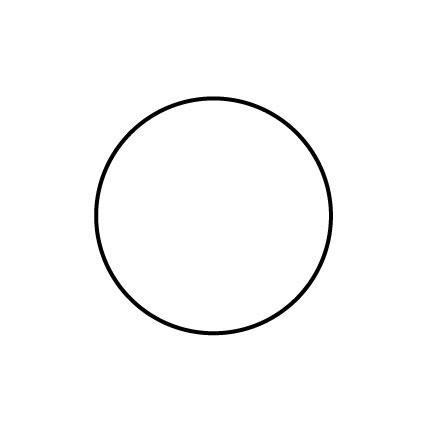
\includegraphics[height = 1.5in]{unknot_1.jpg} 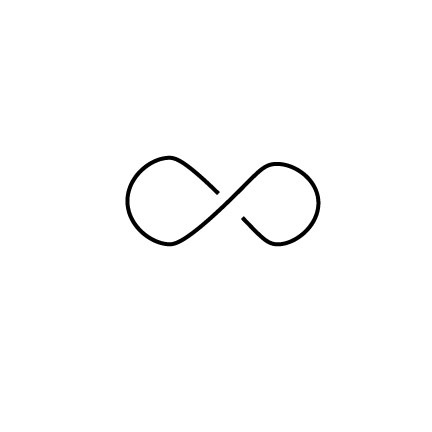
\includegraphics[height = 1.5in]{unknot_2.jpg} 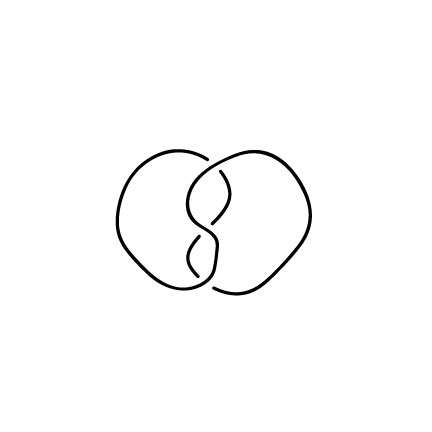
\includegraphics[height = 1.5in]{unknot_3.jpg}
\item Left-handed Trefoil:\\
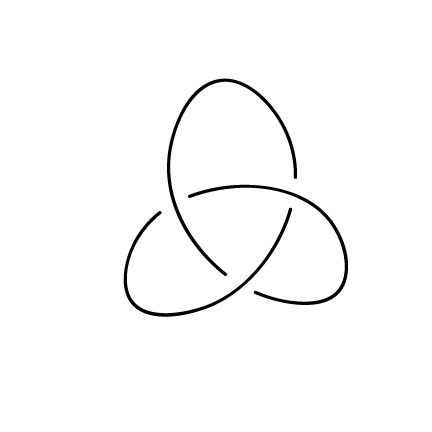
\includegraphics[height = 1.5in]{left_handed_trefoil_1.jpg} 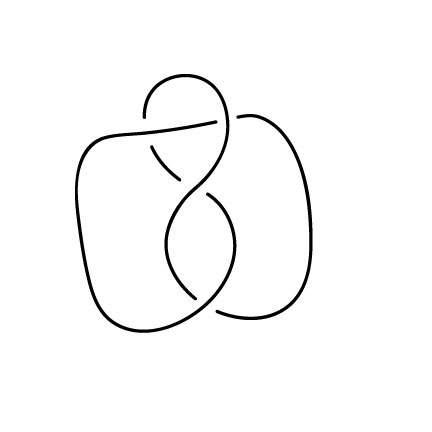
\includegraphics[height = 1.5in]{left_handed_trefoil_2.jpg} 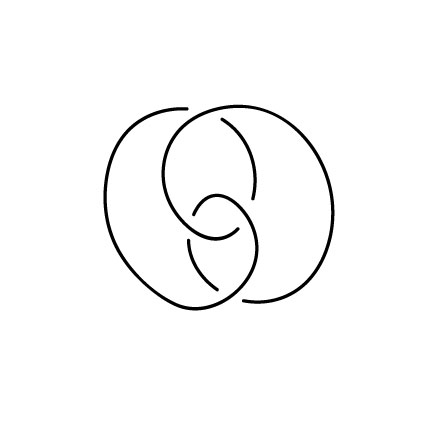
\includegraphics[height = 1.5in]{left_handed_trefoil_3.jpg} 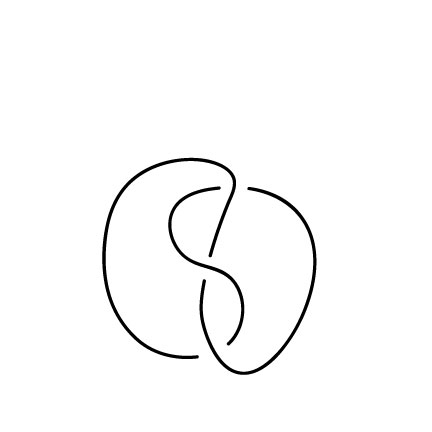
\includegraphics[height = 1.5in]{left_handed_trefoil_4.jpg}
\item Right-handed Trefoil:\\
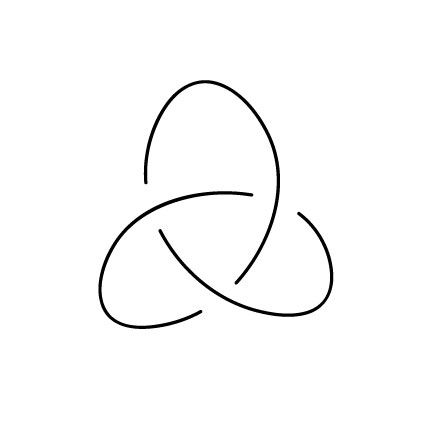
\includegraphics[height = 1.5in]{right_handed_trefoil.jpg}
\item Hopf Link:\\
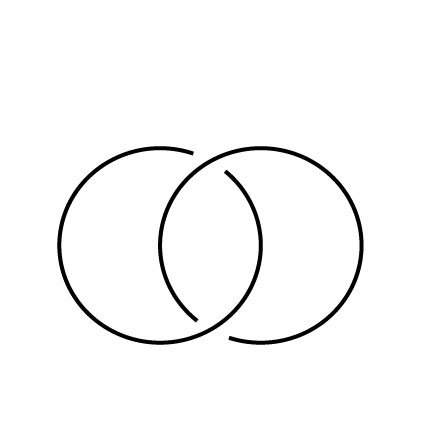
\includegraphics[height = 1.5in]{hopf_link.jpg}
\item Borromean Rings:\\
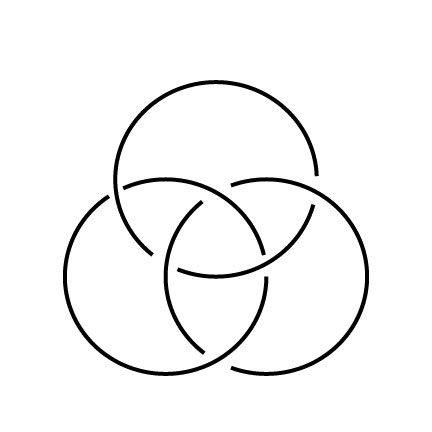
\includegraphics[height = 1.5in]{borromean_rings.jpg}
\item Figure-eight knot:\\
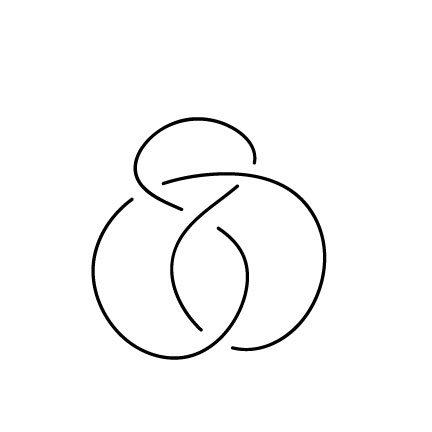
\includegraphics[height = 1.5in]{figure_eight_1.jpg}
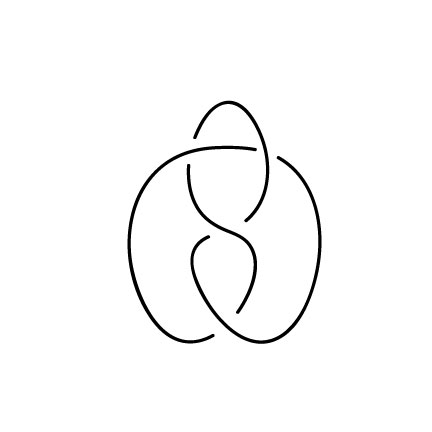
\includegraphics[height = 1.5in]{figure_eight_2.jpg}
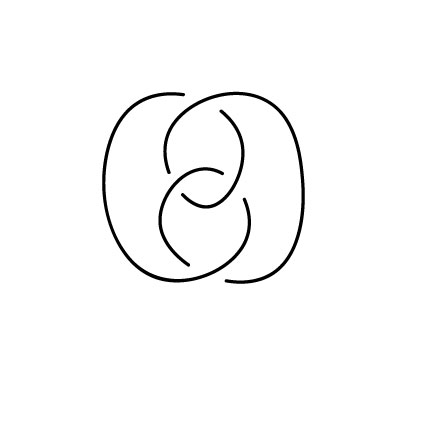
\includegraphics[height = 1.5in]{figure_eight_3.jpg}
\item Square knot:\\
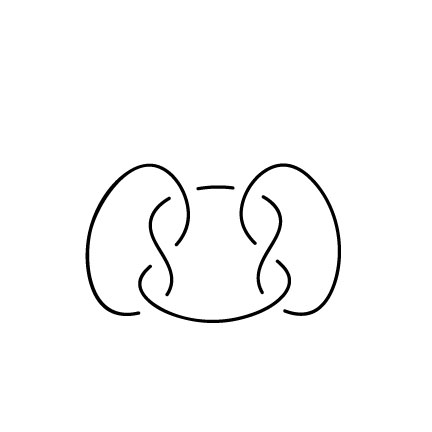
\includegraphics[height = 1.5in]{square_knot_1.jpg}
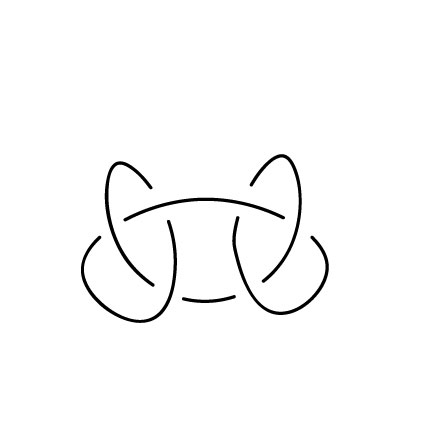
\includegraphics[height = 1.5in]{square_knot_2.jpg}
\end{itemize}

Note that some knots have several different diagrams which look very different (such as the trefoils and figure-eight knots), and some diagrams which look similar turn out to be different knots. For example, the left-handed and right-handed trefoil knots are actually different knots! We will learn how to show this soon. Along those lines, it may seem obvious that some knots aren't equivalent to the unknot (i.e. can't be untied without cutting and reattaching), but this needs to be proved. You will learn how to do this as well!

For the knot diagrams we've seen so far, it may seem like these questions are not too hard to answer. However, as knot diagrams get more crossings, a naive study of them gets much more difficult.

\begin{exercise}
The following knot is the unknot. Try to see why, or at least enough to see that it is a hard question. (Note that this is a difficult task.)
\vspace{.2in}
\begin{center}
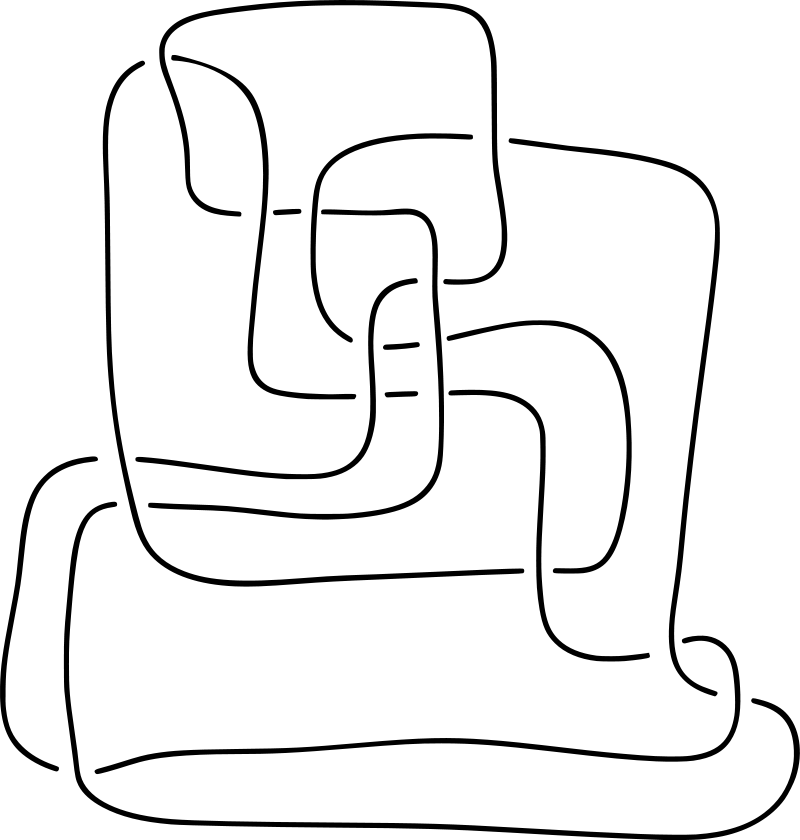
\includegraphics[height = 2in]{tricky_unknot.png}
\end{center}
\end{exercise}

In fact, it was a big problem in knot theory to even be able to detect if a knot is the unknot. Tools now exist, but it takes some surprisingly sophisticated mathematics to do so!

\subsection{Reidemeister Moves}

It can be hard to see if two knot diagrams represent the same knot! Luckily, we have some simple rules for manipulating knots to see whether or not their knot diagrams are the same; these are called the \textbf{Reidemeister\footnote{Pronounced RHY-duh-my-ster.} moves}. They are:

\begin{enumerate}
\item[R1]:\\
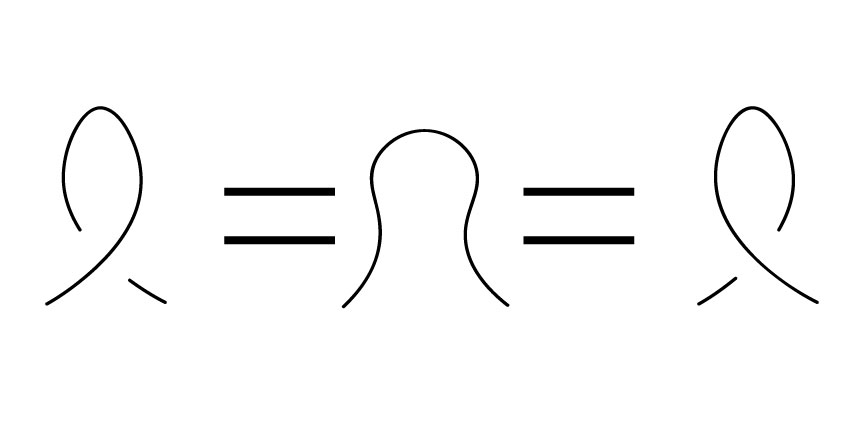
\includegraphics[height = 1.5 in]{reidemeister_1.jpg}
\item[R2]:\\
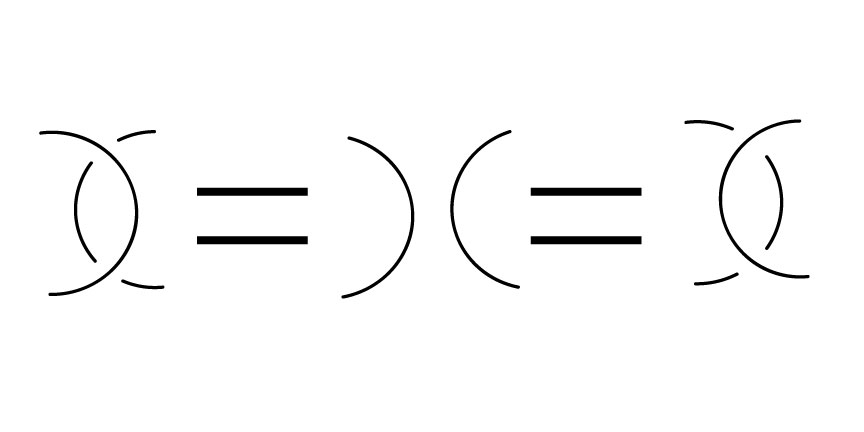
\includegraphics[height = 1.5 in]{reidemeister_2.jpg}
\item[R3]:\\
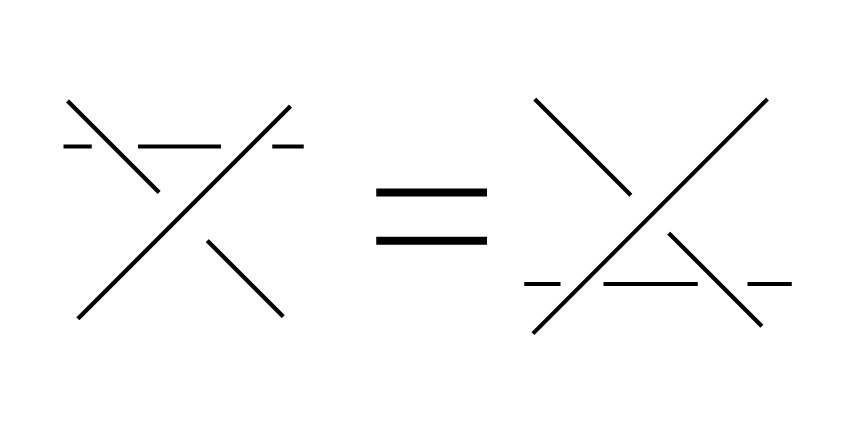
\includegraphics[height = 1.5 in]{reidemeister_3.jpg}
\end{enumerate}

It's easy to see that these moves don't change the knot. What is surprising though is that these are the only 3 moves you'll ever need! In other words, if two diagrams are the same, they are related by a sequence of these three moves.

\begin{exercise}Take a pipe cleaner or piece of string, tie it into a random knot, and connect the ends. Draw the knot diagram for this knot. Is it equivalent to one of the knots given above? Try this with a few different random knots.
\end{exercise}
\begin{exercise}Use the three Reidemeister moves to show that the diagrams of the unknot shown are the same.
\end{exercise}
\begin{exercise}Use the three Reidemeister moves to show that the diagrams of the left-handed trefoil are the same.
\end{exercise}
\begin{exercise}Use the three Reidemeister moves to show that the diagrams of the figure-eight knot are the same.
\end{exercise}
\begin{exercise}Does the square knot look like it has parts of it similar to any of the other knots shown in the examples? In other words, are there any portions of the square knot that, when pinched off and isolated, look like another knot?
\end{exercise}

You may want to play with some pipe cleaner or string to help answer the above exercises. Also, you may think that the left-handed and right-handed trefoil knots are the same. Play with your pipe cleaner or string for long enough and you may see that they might actually not be. As is, we have no way of proving that they are different, or even that neither is equivalent to the unknot. With some more tools and machinery, we will be able to!



\newpage
\section{The Bracket Polynomial}

As you probably noticed, it can be very hard to deduce properties of knots by studying their diagrams, like ``are these two diagrams describing the same knot?", ``is this knot equal to its mirror image?" (remember, this was true for the figure-8 knot but not the trefoil), and even ``is this diagram describing the unknot?". In this section, we will find a powerful tool to help us answer these difficult questions, at least partway.

\subsection{Polynomial Invariants}
First, let's recall what a polynomial is. A polynomial is a mathematical expression of the form $a_n x^n + a_{n-1}x^{n-1} + \cdots + a_1 x + a_0$, where the $a_i$'s are real numbers and the $x$'s are variables. Some examples of polynomials are $x^2 + x + 1, 3x - 2, x^3 - x^2 + 8$ and $\pi x^{39} - \sqrt{2} x^{23} + \frac{17}{307} x^4$.

The idea of a polynomial invariant is that, for a diagram $D$ of a knot $\mathcal{K}$, we want to find a way to assign a polynomial expression $J(D)$ to $D$ in such a way that \textit{any} diagram of $\mathcal{K}$ takes the same value $J(D)$. For example, two diagrams $D_1$ and $D_2$ for the unknot, such as
\begin{center}
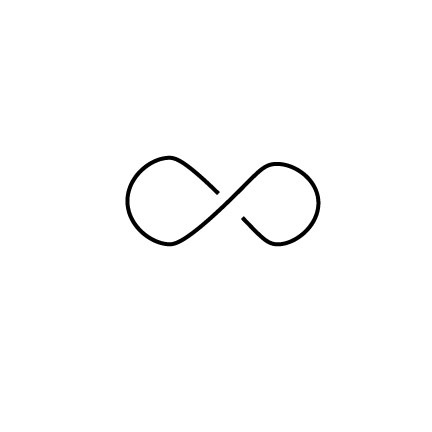
\includegraphics[height = 1in]{unknot_2.jpg}\quad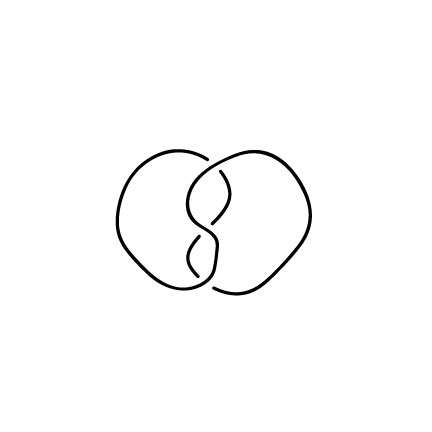
\includegraphics[height = 1in]{unknot_3.jpg}
\end{center}
would give rise to polynomials $J(D_1)$ and $J(D_2)$. Our goal is to define these polynomials so that $J(D_1)=J(D_2)$. Another way of thinking of this is the following: if we have two diagrams $D_1,D_2$, with $J(D_1)\neq J(D_2)$, then $D_1$ and $D_2$ must describe two different knots. This will give us a tool to at least answer when two knot diagrams are describing different knots.

Note that by the Reidemeister Theorem we only need to check that the polynomial $J$ doesn't change under the three Reidemeister moves. In other words, if we start with a diagram $D_1$, apply a Reidemeister move to it to get a new diagram $D_2$, then we want $J(D_1)=J(D_2)$. We'll eventually define $J$ so that it satisfies everything we want it to satisfy, but first we need to introduce the {\bf bracket polynomial}.

\subsection{Finding the Bracket Polynomial}

For a knot diagram $D$ we will assign a mathematical expression with symbol $\langle D\rangle$, called the \textbf{bracket polynomial} of $D$, by a number of rules. The bracket works by modifying each crossing in the diagram, so that we are eventually left with a collection of (unlinked) unknots; this is the first rule below. The next two rules tell us how to simplify the bracket with respect to unknots in the diagram. Expressed mathematically, the rules are as follows.  Note that $O$ represents the unknot below.
\begin{enumerate}
\item[1]: \\ 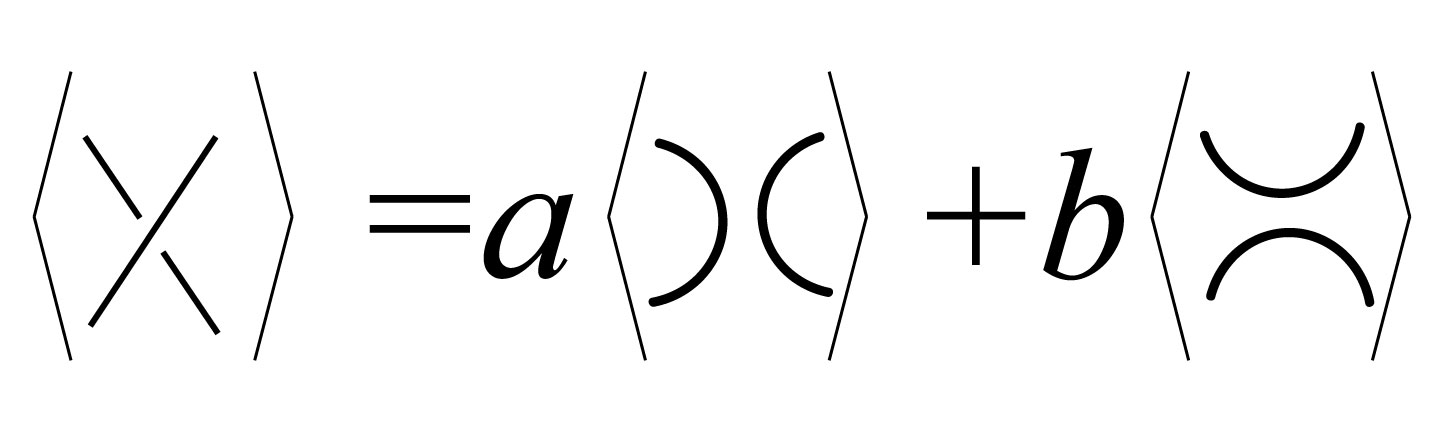
\includegraphics[height = 0.5in]{bracket_1.jpg}
\item[2]: $\langle D O\rangle = c\langle D\rangle$
\item[3]: $\langle O\rangle = 1$.
\end{enumerate}

This notation certainly looks strange! It requires some practice and getting used to. Rule 1 describes how to handle each crossing in a knot diagram. Specifically, it explains how to untie each crossing in the knot diagram. 

Imagine having a knot diagram with multiple crossings, focus on a single crossing at the time; the $=$ sign in rule 1 means that such crossing can be replaced with the two pictures on the right hand side of rule 1. These two pictures are showing the two possible ways we have of untying a crossing. First, think of untying it in one direction (``horizontal") - that's what is shown in the figure with a, and then imagine untying it in the other direction (``vertical") - that's what's shown in the figure with b. 

We would then repeat this process for all the other crossings in our knot diagram until we are left with no crossings. By applying this procedure to each crossing, we obtain a mathematical expression representing our knot diagram made by a sum of terms (depending on a and b) that come from untying the various crossings in our knot. At this point, we would use rule 2 and 3 to remove all the circles left in our diagram. 

Let's see if we can make things clearer with an example. We can compute the bracket polynomial of a ``twisted unknot". This knot has only one crossing, as shown below. The most difficult step in the process is getting rid of said crossing (this is described in the first line of the example): we separate the crossing by using rule 1 and replacing it in the knot diagram in two ways, either horizontally ($a$ term) or vertically ($b$ term). Then we use rule 2 to get rid of one of the circles in the first term (that's how $c$ appears in the second line). Finally, we use rule 3 to ``absorb" the leftover unknots (third line).
\\
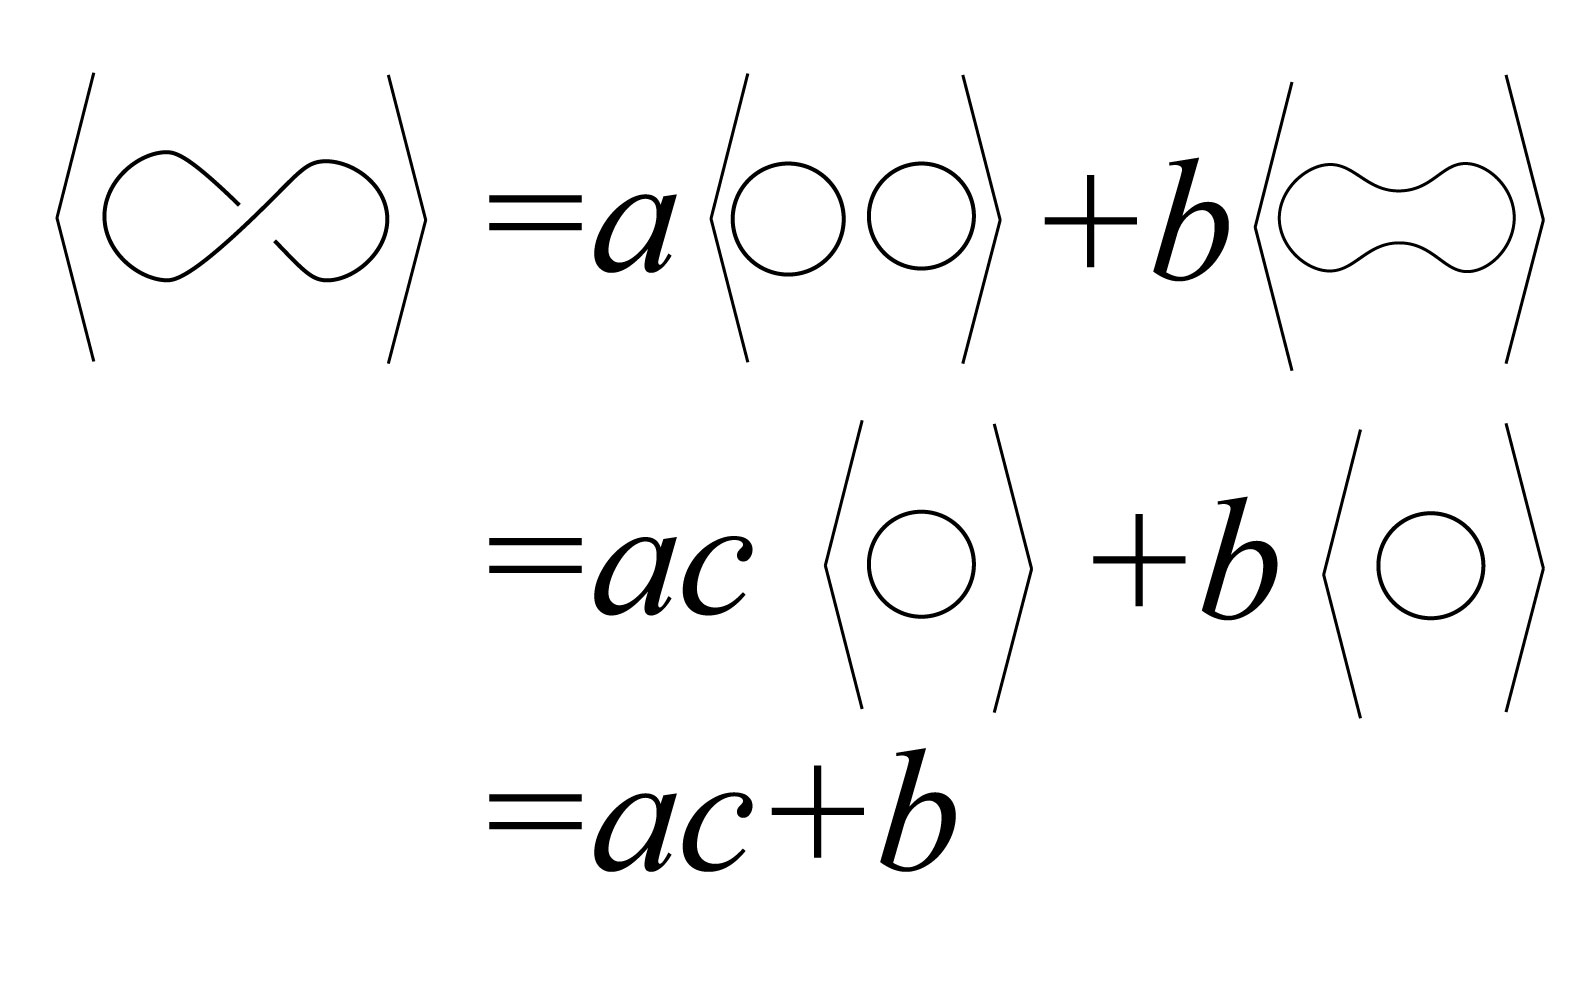
\includegraphics[height = 2in]{unknot_bracket_comp.jpg}

Hence, the idea with finding the bracket polynomial $\langle\,\,\rangle$ of a knot is that we'll eventually get rid of all the crossings of the knot diagram $D$ and be left with some expression involving $a,b,$ and $c$ only. To see that this will always happen, note that, since each rule transforms our knot into something closer to a circle or a link of circles, our knot will eventually consist of a bunch of $a$'s, $b$'s, and $c$'s multiplied with $\langle O\rangle = 1$ (rule 3). 

\begin{exercise}
Compute the bracket polynomial of the following diagram of the Hopf link:
\begin{center}
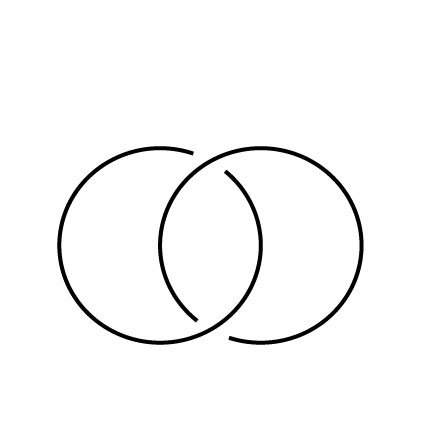
\includegraphics[height=1in]{hopf_link.jpg}
\end{center}
\end{exercise}

Another point worth mentioning about rule 1: if the crossing you're considering in your knot diagram, as it's drawn, doesn't match up with the left-hand side of rule 1, we rotate the diagram until the crossing does match up with rule 1 and apply the rule. One way to think of this is to think of walking along the top strand of a crossing. When you reach the crossing, turn to the left and multiply by $a$ and throw in the other strand; then add a term where you turn to the right, throw in the other strand and multiply by $b$. Either way you're walking on the top strand, turning to the left will give the same two strands, so it doesn't matter whether you think of walking along the top strand ``top to bottom" or ``bottom to top." Before moving on to the next section, consider watching the video titled {\it Example: Bracket Polynomial of the Hopf Link} on our website: https://girlstalkmath.com/knot-theory/.

\subsection{Refining the Bracket Polynomial}

As it stands, the bracket polynomial gives a polynomial in three variables: $a,b,c$. It would be really nice to have a polynomial in only one variable. But also notice that the rules we used to define the bracket polynomial ``doesn't see" much information about the knot. For example, it doesn't ``see" if diagrams represent the same knot. Let's see if we can solve both of these problems at the same time! In other words, can we pick $a,b,c$ in a special way such that the bracket polynomial becomes a polynomial in only one variable \textbf{and} can ``see" Reidemeister invariance? The answer is yes!

If we want the bracket polynomial to detect Reidemeister invariance, we would want the following three equalities to hold:

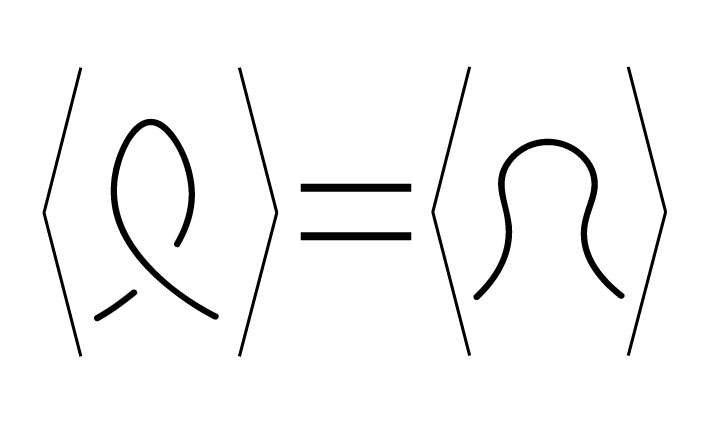
\includegraphics[height = 0.5in]{bracket_equal_3.jpg},
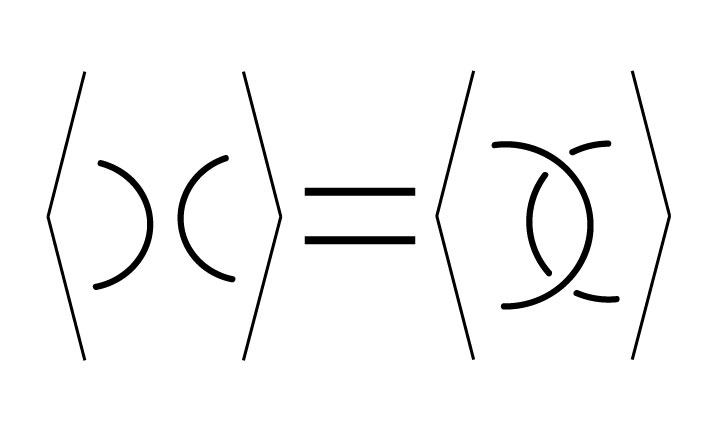
\includegraphics[height = 0.5in]{bracket_equal_1.jpg},
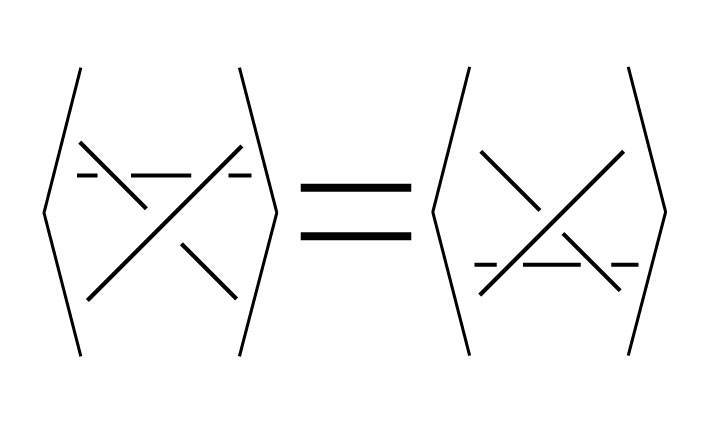
\includegraphics[height = 0.5in]{bracket_equal_2.jpg}.

Before trying the process on your own, consider watching the video {\it Example: Reidemeister Moves} on our website at https://girlstalkmath.com/knot-theory/.

\begin{exercise} \label{ex:brack}
Compute the following bracket:\\

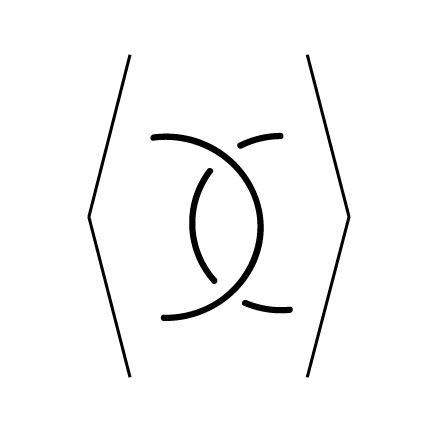
\includegraphics[height = 0.5in]{bracket_equal_1-2.jpg}.\\

Note that this knot diagram has two crossings and once you compute the bracket polynomial for it you will have some multiples of two brackets with no crossings multiplied by some terms involving $a,b,c$. Solve your bracket expression for $b,c$ (in terms of $a$) so that it is equal to the (already fully simplified bracket)
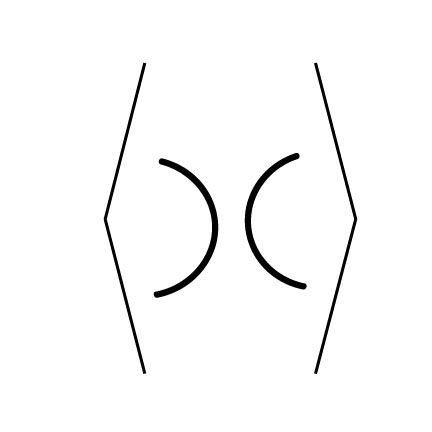
\includegraphics[height = 0.5in]{bracket_equal_1-1.jpg}.

This problem can be tricky at first because the notation is unusual.

This forces $\langle\,\,\rangle$ to be invariant under $R2$; in other words, if $D_1$ and $D_2$ are diagrams which differ only by applying a single $R2$ move, then $\langle D_1\rangle =\langle D_2\rangle$. Go back to the beginning of this section and replace $b,c$ in the definition of the bracket polynomial with the values you found (in terms of $a$) in this exercise.
\end{exercise}

\begin{exercise} \label{ex:brack2}
Using the values for $b,c$ you found in Exercise 2.\ref{ex:brack}, compute the following brackets:\\
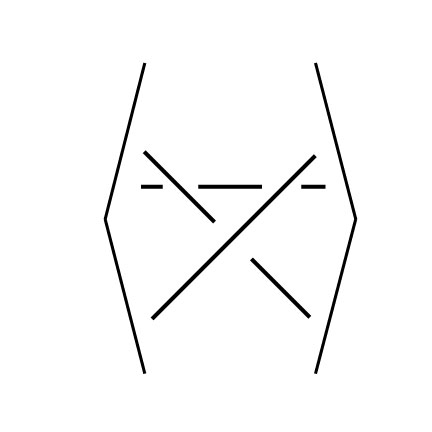
\includegraphics[height = 0.5in]{bracket_equal_2-1.jpg}, 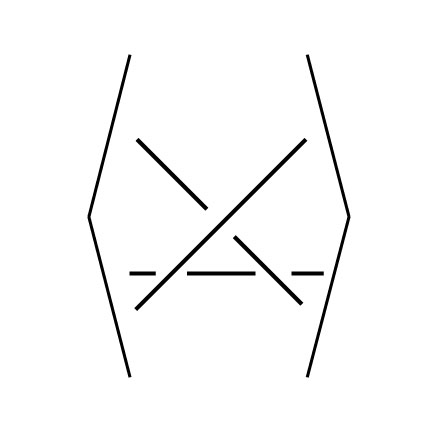
\includegraphics[height = 0.5in]{bracket_equal_2-2.jpg}.\\

Hint: You only need to apply the bracket rules to the middle crossing! You are allowed to use that the bracket is R2-invariant, because in Exercise 2.\ref{ex:brack2}, we picked $b,c$ that would make it R2-invariant.

Is the bracket polynomial invariant under $R3$?
\end{exercise}

\begin{exercise}
	Finally let's (try to) check $R1$-invariance. Compute the brackets:\\
	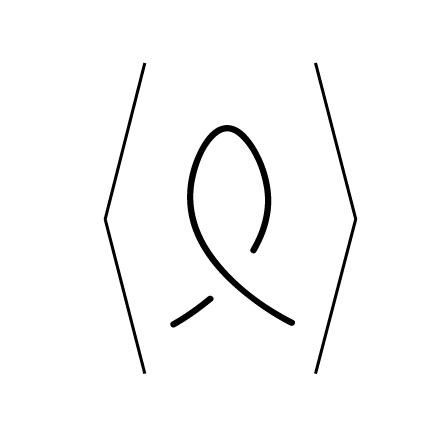
\includegraphics[height = 0.5in]{bracket_equal_3-1.jpg}, 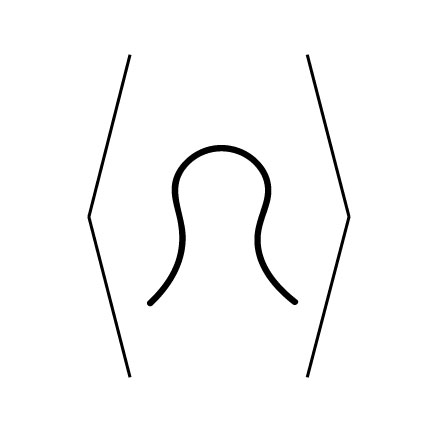
\includegraphics[height = 0.5in]{bracket_equal_3-2.jpg}.
	
Is the bracket polynomial $\langle \rangle$ invariant under $R1$? Spoiler alert: it's not, unless we pick $a$ such that $a^3=-1$. Why do you think this condition would be enough to guarantee $R1$-invariance? Use what you found above to verify that this would indeed make the bracket polynomial invariant under $R1$. 
\end{exercise}

Although we now know that this condition on $a$ would make the bracket polynomial $R1$-invariant, we choose not to apply this substitution because it's a huge restriction on the possible values of our constants. Doing so would force $a=-1$ (or $a$ would need to be a complex number), and this would change our invariants to be numbers rather than polynomials. We will find a way around this issue in the next section.  

We were really hoping that the bracket polynomial would be invariant under all three Reidemeister moves; if that was the case, we could have used it to figure out whether or not two diagrams (and hence the knots they represent) were different. But all is not lost! It turns out the bracket polynomial is a really good start (it works for 2 out of 3 of the Reidemeister moves), and soon we'll modify it to achieve our goal. With this in mind, let's get a little more familiar with it.

\subsection{Exercises}

\begin{exercise}
	Above we computed the bracket polynomial for a twisted unknot. Now try computing the bracket polynomial for an unknot with two twists:\\
	\begin{center}
	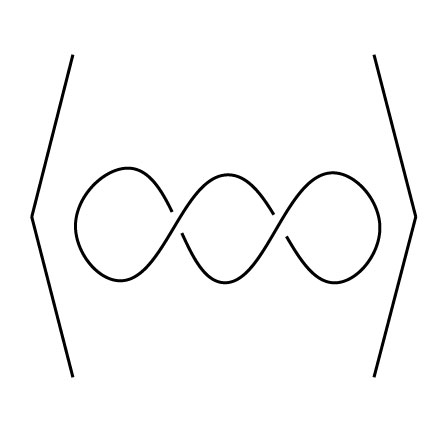
\includegraphics[height = 1in]{exercise_4.jpg}	
	\end{center}
\end{exercise}

\begin{exercise}
	Compute the bracket polynomial for the Hopf link with diagram
	\begin{center}
	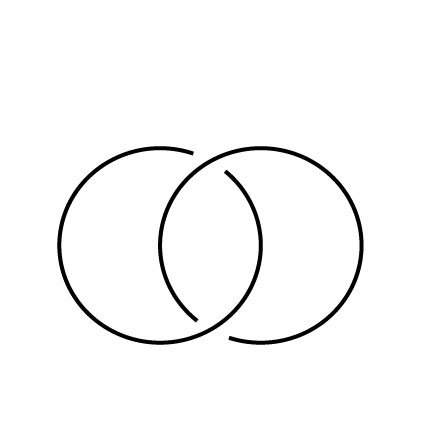
\includegraphics[height=1in]{hopf_link.jpg}
	\end{center}
\end{exercise} 

\begin{exercise}
	Compute the bracket polynomial for the left-hand trefoil with diagram
	\begin{center}
	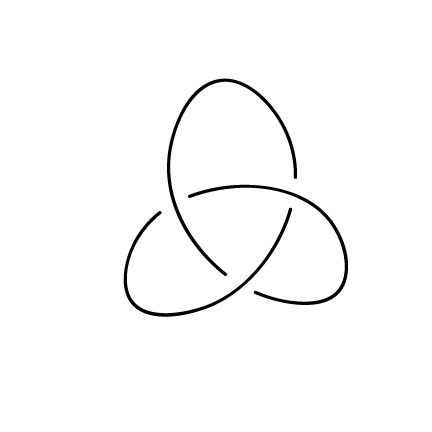
\includegraphics[height=1in]{left_handed_trefoil_1.jpg}
	\end{center}
\end{exercise}

\begin{exercise}
	Compute the bracket polynomial for the right-hand trefoil with diagram
	\begin{center}
	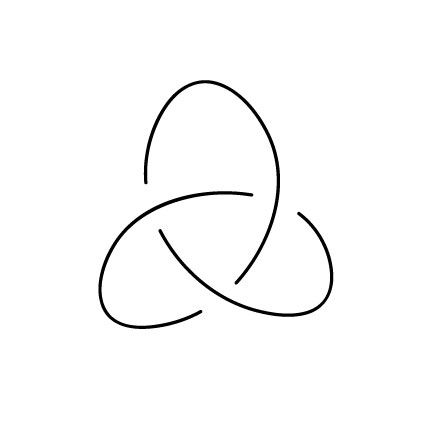
\includegraphics[height=1in]{right_handed_trefoil.jpg}
	\end{center}
\end{exercise}

\begin{exercise}
	What did you notice about the exercises focused on the two trefoils? Do you notice a pattern? Do you think this pattern holds in general? Why or why not?
\end{exercise}

\newpage
\section{The Jones Polynomial}

The bracket polynomial was \textit{almost} able to distinguish knots from each other, but wasn't invariant under the first Reidemeister move. In this section, we'll modify the bracket polynomial by introducing some other tools and techniques to make it invariant under all the Reidemeister moves! Because two diagrams represent the same knot when they differ only by some of the three Reidemeister moves, being invariant under all three Reidemeister moves means that \textit{any} diagram of a given knot (or link) will have the same polynomial representation. With this tool in hand, we will finally be able to tell some knots apart!

\subsection{Review of the bracket polynomial}
To begin, recall that for a knot diagram $D$, its bracket polynomial $\langle D\rangle$ could be computed via the following rules (where $O$ denotes the unknot):
\begin{enumerate}
\item[1]:\\
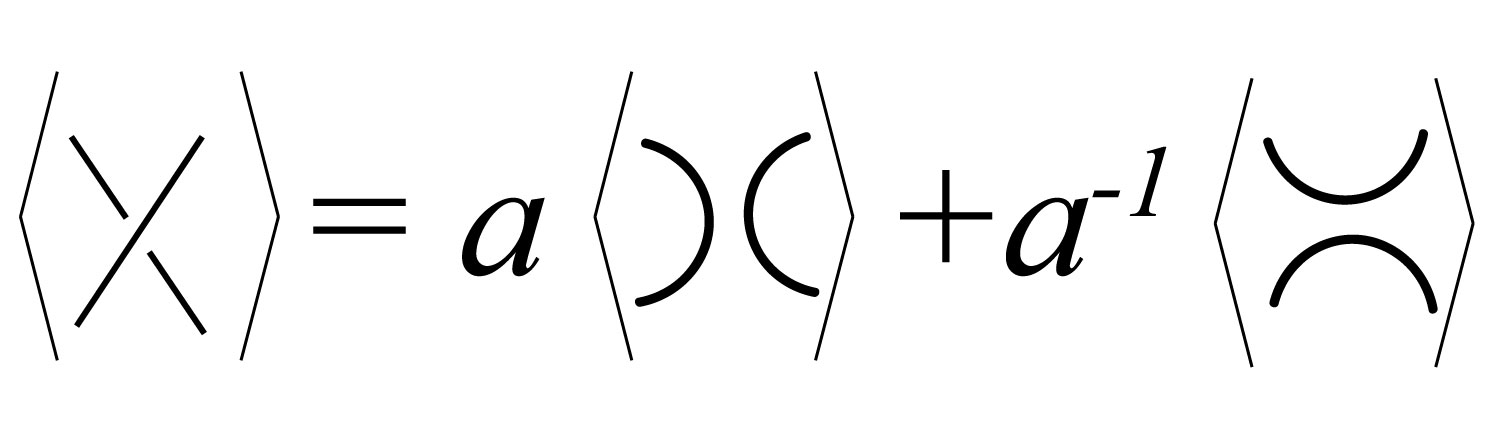
\includegraphics[height = 0.5in]{bracket_1_true.jpg}
\item[2]: $\langle D\,O\rangle=(-a^2-a^{-2})\langle D\rangle$
\item[3]: $\langle O\rangle=1.$
\end{enumerate}

We chose the rules above so that $\langle\,\,\rangle$ is invariant under $R2$ and $R3$. Unfortunately the bracket polynomial is not invariant under $R1$, since the bracket changes by $-a^{\pm3}$ (Exercise 2.4). To correct the bracket polynomial so that it has R1 invariance we need to introduce a few more concepts to lead us to the Jones polynomial, which will be invariant under R1, R2, and R3. 

\subsection{Positive and negative crossings}
First, we will need to \textit{orient} our knots. An \textbf{orientation} for a knot is, roughly speaking, a choice of direction to travel along the knot. In practice one draws an arrow pointing in one of the two possible directions, and for easy visualization draws a few more arrows in other places along the knot. 

In what follows, the way we orient a knot won't actually matter. For links though, orienting parts of the link in different ways may give distinct links. For example, we will show that these two oriented links are different:\\
\begin{center}
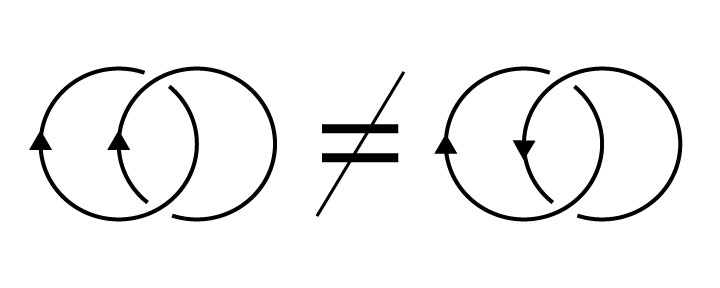
\includegraphics[height=1in]{hopf_not_equal.jpg}
\end{center}

We now define a positive and a negative crossing. A positive crossing is one which agrees with the so-called ``right-hand rule." Using your right hand, if you put your fingers pointing along the arrow of the top strand of a crossing, and then curl your fingers towards the outcoming arrow of the bottom strand of a crossing, the crossing is positive if your thumb points towards you and the crossing is negative if your thumb points away from you (the picture below will help). We now define the Writhe number of a crossing by $w(x)=1$ if $x$ is a positive crossing and $w(x)=-1$ if $x$ is a negative crossing. In (much easier to understand) symbols,\\
\begin{center}
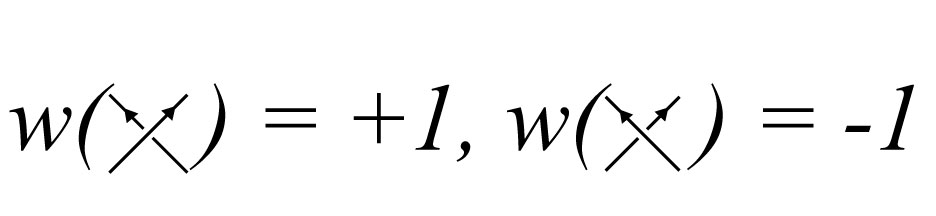
\includegraphics[height=1in]{writhe_definition.jpg}
\end{center}

If an oriented crossing doesn't exactly match up with one of the two crossings above, we can rotate the diagram so that it does (or use the right-hand rule). When computing $w$ of a crossing $x$, it may be helpful to turn the paper (or your head) so that both arrows are pointing up. Then, if the strand on top moves from left to right, $w(x)=+1$; otherwise, $w(x)=-1$.

Next, for an oriented diagram $D$, we set $w(D)$ to be the sum of $w(x)$ for each crossing $x$ of $D$; in other words, we let $w(D)$ be the difference between the positive and negative crossings. As an example, we compute the Writhe number of the oriented left-handed trefoil:\\
\begin{center}
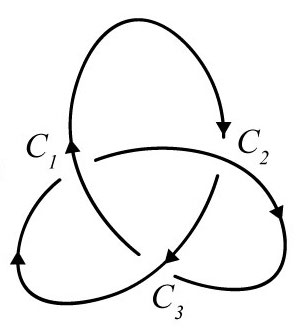
\includegraphics[height=1in]{trefoil_writhe_example.jpg}
\end{center}

There are three crossings $C_1, C_2,$ and $C_3$, with Writhe numbers: $w(C_1) =-1, w(C_2) = -1,$ and $w(C_3) = -1$. Thus, $w = w(C_1) + w(C_2) + w(C_3) = -3$.

\begin{exercise}
	Compute the Writhe numbers for the oriented Hopf links shown above. Remember that orientation here matters; how does choice of orientation affect the Writhe number?
\end{exercise}

\begin{exercise}
	Compute the Writhe number of the diagram of the right-handed trefoil that is the mirror image of the diagram of the left-handed trefoil in the example above. Is it the same as or different to the Writhe number of the diagram of the right-handed trefoil shown above?
\end{exercise}

\begin{exercise}
	For a knot diagram, there are exactly two orientations. Why will either orientation give the same Writhe number? (Hint: draw a positive crossing and consider what would happen if the orientation were reversed; is it still a positive crossing?)
\end{exercise}

\begin{exercise}
	Show that the Writhe number $w$ is invariant under Reidemeister moves $R2$ and $R3$ by computing the Writhe number for appropriate choices of crossings (look at the crossings used to define $R2$ and $R3$). Is $w$ invariant under $R1$?
\end{exercise}

\subsection{Defining the Jones Polynomial}
From the previous exercise, we see that $w$ is invariant under $R2$ and $R3$, but not $R1$. This was true of the bracket polynomial as well. Could there be a clever way to use both of these to build a polynomial which actually is invariant under all the Reidemeister moves? The answer is yes! To do this, we define the \textbf{Kauffman polynomial} $X(D)$ for the knot of diagram $D$ as:
$$X(D)=(-a)^{-3w(D)}\langle D\rangle.$$
Note that to compute $w(D)$ we need an orientation on $D$, but to compute $\langle D \rangle$ we don't: when you compute $\langle D\rangle$ and $D$ has an orientation, you ignore the orientation.

As an example, we can compute the Kauffman polynomial of the left-handed trefoil $\mathcal{T}_{lh}$. Above we computed $w(\mathcal{T}_{lh}) = -3$ for this knot, and from a previous exercise we know that $\langle \mathcal{T}_{lh}  \rangle = a^{7} - a^{3} - a^{-5}.$ Thus, the Kauffman polynomial of $T$ is:
\begin{align*}
	X(\mathcal{T}_{lh}) 	&= (-a)^{-3w(\mathcal{T}_{lh})} \langle\mathcal{T}_{lh}\rangle\\
			&= (-a)^{-3\cdot(-3)}(a^{7} - a^{3} - a^{-5})\\
			&= (-a)^9(a^{7} - a^{3} - a^{-5})\\
			&= -a^{16} + a^{12} + a^{4}.
\end{align*}

\begin{exercise}
Show that the Kauffman polynomial is invariant under all three Reidemeister moves. Hint: you only need to show that $X(D_1) = X(D_2)$, when $D_1$ and $D_2$ differ by an $R1$ move, since we can assume invariance under $R2$ and $R3$. Why can we make this assumption?
\end{exercise}

\begin{exercise} Suppose we're given knot diagrams $D_1$ and $D_2$. If $X(D_1)\neq X(D_2)$, can $D_1$ and $D_2$ be diagrams of the same knot? Why or why not?
\end{exercise}

\begin{exercise} Compute $X($unknot$)$ and $X($right-handed trefoil$)$. Using this and the previous exercise, is it possible to untie the trefoil (without cutting the string)?
\end{exercise}

We are finally ready to define the Jones Polynomial $J(\mathcal{K})$ (and basically already have). To do this, we compute $X(D)$ for a diagram of the knot (or link) $\mathcal{K}$ and substitute $a=q^{-1/2}$. This may seem silly, but there are historical reasons for this substitution: the Jones polynomial was initially defined in a different way, and this (equivalent but simpler) way of defining it was discovered just a couple years later. The Jones polynomial is such a powerful tool that it won a Fields Medal, which is the mathematics equivalent of a Nobel Prize.

We note that there is a way to re-write the relations to define the Jones polynomial directly without going through the bracket polynomial. Unfortunately, doing so is lengthy, not straightforward, and muddies the intuitive approach we made through the bracket polynomial for little gain; we therefore omit that formulation.

\subsection{Skein relation}
An alternate way to compute the Jones polynomial is via the following Skein relation\footnote{To prove this, first prove an analogous identity for the bracket polynomial, and then think about what happens to the Writhe numbers. This proof is quite a challenge at this point. However, this was the formulation which Jones originally gave for computing the polynomial, and it often is quicker to compute this way.}
\begin{center}
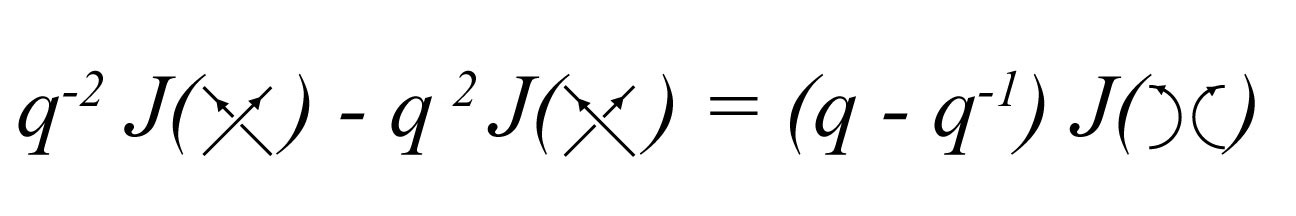
\includegraphics[height = .5in]{jones_property.jpg}
\end{center}
along with the rules
$$J(D\,O)=-(q^{-1}+q)J(D),\quad J(O)=1.$$
This can make computing the Jones polynomial much faster. If we pick a crossing strategically and apply the Skein relation, one term switches the crossing, which may simplify the knot significantly (maybe even to the unknot), and another term has one fewer crossing. Note that, as before, you may need to rotate the picture to get the crossings pictured as shown. Before working on the following exercises, consider watching the video {\it Example: Skein Relation} on our website at https://girlstalkmath.com/knot-theory/.

\subsection{Exercises}

\begin{exercise}
Compute the Jones polynomials of the two Hopf links with different orientations shown earlier in this problem set.
\end{exercise}

\begin{exercise}
Use the above relations to compute the Jones polynomial of the right-handed trefoil. (Note that you will need the Jones polynomial of the Hopf link with a certain orientation partway through). Note that we computed the Jones polynomial of the left-handed trefoil in an earlier example. What can you conclude about the left-handed and right-handed trefoils?
\end{exercise}

The \textbf{mirror image} $\overline{\mathcal{K}}$ of a knot $\mathcal{K}$ is defined to be (naturally enough!) the knot obtained by looking at the mirror image of a knot diagram. For example, the left-handed trefoil is the mirror image of the right-handed trefoil. From the computation above, we see that the Jones polynomial of the mirror image of the trefoil knot is almost the same polynomial, but with $	q$ replaced by $q^{-1}$. This property always holds.

\begin{exercise}
Show that if $\overline{\mathcal{K}}$ is the mirror image of a knot $\mathcal{K}$, then $J(\overline{\mathcal{K}})$ is $J(\mathcal{K})$ with $q$ replaced by $q^{-1}$.
\end{exercise}

\begin{exercise}
Compute the Jones polynomial of the figure-eight knot, using either diagram below (they both represent the same knot).
\begin{center}
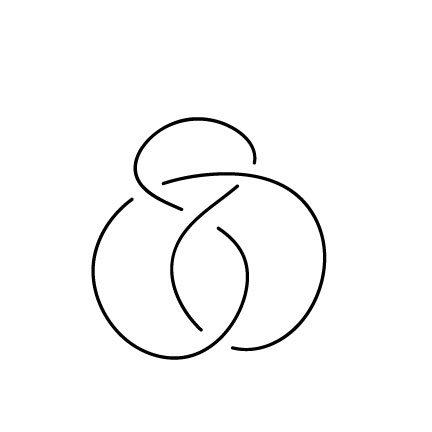
\includegraphics[height=2in]{figure_eight_1.jpg}
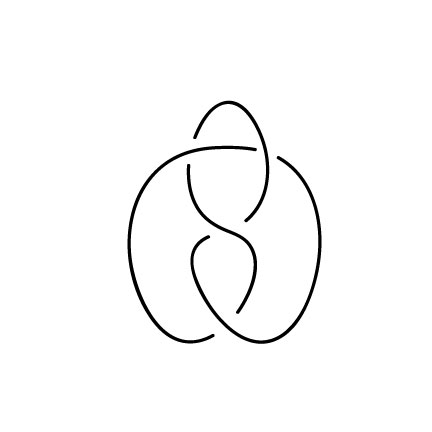
\includegraphics[height=2in]{figure_eight_2.jpg}
\end{center}
Unlike the (left-handed) trefoil, the figure eight knot \textit{is} equal to its mirror image. How is this fact reflected in its Jones polynomial?
\end{exercise}

\begin{exercise}
Compute the Jones polynomial (in any way you choose) of the \textbf{square knot}. Two diagrams of the square knot are shown below.\\
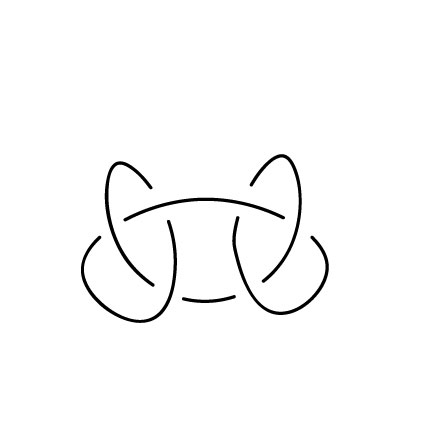
\includegraphics[height=2in]{square_knot_2.jpg}
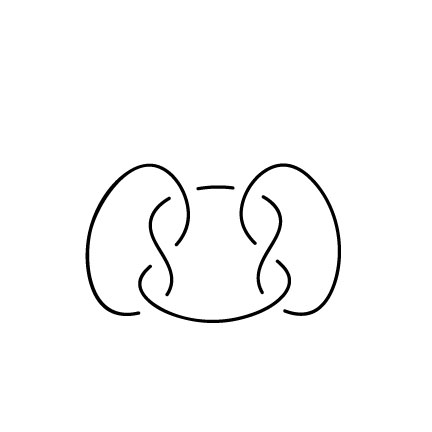
\includegraphics[height=2in]{square_knot_1.jpg}
\end{exercise}



\newpage
\section{Knot Algebra}
Given two knots\footnote{Throughout, we've been using the terms ``knot" and ``link" somewhat interchangeably. Here, it is important that we are actually talking about knots, meaning they are only one piece of ``string tied up".} $\mathcal{K}_1,\mathcal{K}_2$, there is a way to get a new knot $\mathcal{K}_1\#\mathcal{K}_2$. This notation is used to describe the knot obtained by imagining to actually tying the knots together with strings.; we could tie $\mathcal{K}_1$ and then tie $\mathcal{K}_2$ in the same string, and call the resulting knot $\mathcal{K}_1\#\mathcal{K}_2$. We call $\mathcal{K}_1\#\mathcal{K}_2$ the \textit{connect sum} of $\mathcal{K}_1$ and $\mathcal{K}_2$ (this is how the $\#$ symbol is read). We show this pictorially as follows:\\
\begin{center}
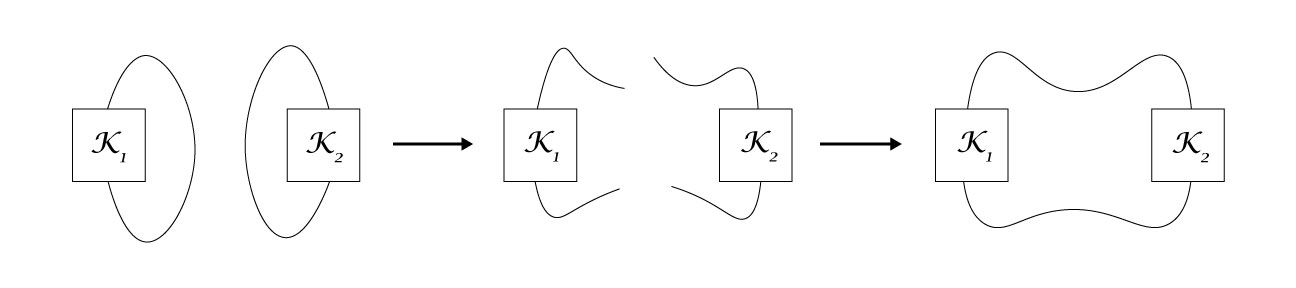
\includegraphics[height = 1.2in]{knot_sum.jpg}
\end{center}
We also comment that connect sum isn't defined in general for links. This is because there is a choice for which ``knot" in the link we would have to ``cut" to form the connect sum. For knots, there is no such ambiguity.

\begin{exercise}
What happens if we take the connect sum with the unknot? In other words, what is $\mathcal{K}\#O$ for any knot $\mathcal{K}$? Hint: think graphically.
\end{exercise}

\begin{exercise}
Suppose we're given knots $\mathcal{K}_1,\mathcal{K}_2$. Is it true that $\mathcal{K}_1\#\mathcal{K}_2 = \mathcal{K}_2\#\mathcal{K}_1$? Why or why not?
\end{exercise}

\begin{exercise}
Does it matter where the knots $\mathcal{K}_1,\mathcal{K}_2$ are originally cut (before you reattach the ends)? Why or why not?
\end{exercise}

\begin{exercise}
Represent the square knot\\
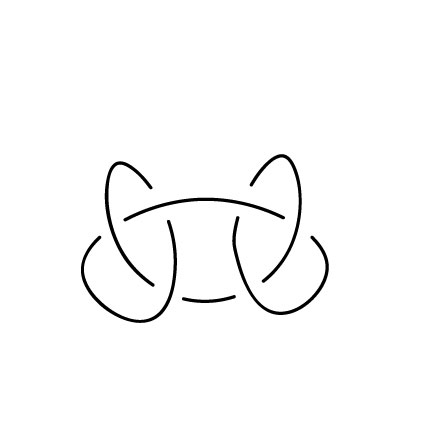
\includegraphics[height=2in]{square_knot_2.jpg}
\includegraphics[height=2in]{square_knot_1.jpg}

\noindent as a connect sum of two other knots. In other words, find two knots such that, when you take their connect sum, you get the square knot. Is this choice unique, or do you think there are multiple pairs? (Spoilers below! Don't read past this!)
\end{exercise}

In fact, the square knot is the connect sum of the left-handed trefoil with the right-handed trefoil. Note that in the last section, we found that:
$$J(\text{left-handed trefoil})=-q^{-8} + q^{6} + q^{2},\quad J(\text{right-handed trefoil})=-q^{-8}+q^{-6}+q^{2}$$
and in an exercise, you computed
$$J(\text{square knot})=(-q^{-8} + q^{6} + q^{2})(-q^{-8}+q^{-6}+q^{2})$$
In general, it is true that $J(\mathcal{K}_1\#\mathcal{K}_2)=J(\mathcal{K}_1)J(\mathcal{K}_2)$.

\begin{exercise}
(Challenge) Use the Skein relation to prove that
$$J(\mathcal{K}_1\#\mathcal{K}_2)=J(\mathcal{K}_1)J(\mathcal{K}_2)$$
Hint: Form the connect sum $\mathcal{K}_1\#\mathcal{K}_2$ with a positive crossing, and apply the Skein relation to this crossing. You may use the fact that
$$J(\mathcal{K}_1\,\,\mathcal{K}_2)=-(q+q^{-1})J(\mathcal{K}_1)J(\mathcal{K}_2)$$
where $\mathcal{K}_1\,\,\mathcal{K}_2$ represents $\mathcal{K}_1,\mathcal{K}_2$ placed beside each other.
\end{exercise}

\subsection{Prime knots}
In the last section, you showed that the square knot is the connect sum of two trefoils. Some knots, however, can't be written this way. For example, there is no way to write the trefoil knot as $\mathcal{K}_1\#\mathcal{K}_2$ unless one of $\mathcal{K}_1$ or $\mathcal{K}_2$ is the unknot; the trefoil is an example of a \textbf{prime knot}. This is analogous to what happens with integers: some integers can be written as the product of two other integers bigger than $1$ (like $6=2\times3$) but others can't (if $7=m\times n$ then one of $m,n$ is $1$). Any knot $\mathcal{K}$ which can be written as the connect sum of $\mathcal{K}_1$ and $\mathcal{K}_2$ ($\mathcal{K} = \mathcal{K}_1\# \mathcal{K}_2$), neither of which is the unknot, is called a \textbf{composite knot}. On the other hand, any knot $\mathcal{K}$ which can be written as the connect sum of $\mathcal{K}_1$ and $\mathcal{K}_2$ ($\mathcal{K} = \mathcal{K}_1\# \mathcal{K}_2$) only if one of them is the unknot (either $\mathcal{K}_1 = O$ or $\mathcal{K}_2 = O$), is called a \textbf{prime knot}.

\subsubsection{Genus}
The \textbf{genus} of a knot is a way of assigning a non-negative integer to a knot in a way that has nice properties. The formal definition is a little beyond what we've covered here, but we have a related concept that's easier to work with (and kinda neat)! Start with a knot $\mathcal{K}$, and our goal will be to treat the knot as the boundary (or edge) of some surface. The way we'll do this is by the following algorithm:

\begin{enumerate}
	\item Pick any diagram $D$ for the knot $\mathcal{K}$, and give $D$ an orientation.
	\item At each crossing, you'll connect the ``incoming'' strand to the adjacent ``outgoing'' strand, similar to what we do in computing the bracket polynomial. This will give you a collection of oriented circles.
	\item Fill in the circles, so you have a collection of disks.
	\item Connect the disjoint disks with bands, so that if you travel along the boundary of a disk (which is oriented), then across the edge of a band, then across the boundary of the attached disk, the orientations should all agree.
\end{enumerate}

The result of this construction is called a \textbf{Seifert\footnote{SIGH-fert.} surface} associated to the knot. Note that, if you use different diagrams $D_1, D_2$ of the same knot $\mathcal{K}$, you may get different surfaces. However, the topic of analyzing these surfaces is a fairly hefty topic that would take more time than we have in this camp.

As an example, we can compute a Seifert surface for the trefoil in four stages:\\
\includegraphics[height = 2in]{seifert_of_trefoil.jpg}

\begin{exercise}
	What is a Seifert surface of the unknot?
\end{exercise}

\begin{exercise}
	What is a Seifert surface of the right-handed trefoil?
\end{exercise}

It's interesting to note that the same construction works for links that are not knots!

\begin{exercise}
	What is a Seifert surface of the Hopf link?
\end{exercise}

\begin{exercise}
	What is a Seifert surface of the Borromean rings? A diagram of the Borromean rings is
	\begin{center}
	\includegraphics[height=1in]{borromean_rings.jpg}
	\end{center}
\end{exercise}

\begin{exercise}
	Let $\mathcal{K}_1, \mathcal{K}_2$ be two knots. How do the Seifert surfaces of $\mathcal{K}_1$ and $\mathcal{K}_2$ relate to the Seifert surface of $\mathcal{K}_1\# \mathcal{K}_2$?
\end{exercise}

Now we can (roughly) talk about the genus $g(\mathcal{K})$ of a knot $\mathcal{K}$, which we mentioned above is a non-negative integer (non-negative means that it could be a positive integer or it could be 0). In general the concept of genus only makes sense for certain kinds of surfaces, but it is useful in the study of knots. With this in mind, mathematicians transformed knots into Seifert surfaces, found the genus of the surface, and then defined the genus of the knot to be the smallest genus of any Seifert surface associated to the knot. Again, we won't work much with the actual genus (including computing it), but we can still work with some properties of it.

\subsubsection{Properties of the genus}
Here listed are some useful facts involving the genus:
\begin{enumerate}
	\item The genus of the unknot is $0$, so $g(O) = 0$. Moreover, the unknot is the \emph{only} not with genus $0$.
	\item The genus behaves well under the operation of connect sum, in that
	$$g(\mathcal{K}_1 \# \mathcal{K}_2) = g(\mathcal{K}_1) + g(\mathcal{K}_2).$$
\end{enumerate}

\begin{exercise}
	Show that a knot of genus $1$ is a prime knot. (Hint: suppose $\mathcal{K}$ has genus $1$ and $\mathcal{K}=\mathcal{K}_1\#\mathcal{K}_2$. What does this imply about the genus of $\mathcal{K}_1$ or $\mathcal{K}_2$?)
\end{exercise}

In particular, one can show that the genus of (either the left-handed or the right-handed) trefoil is $1$. Thus, the trefoil is prime.

\begin{exercise}
	What is the genus of the square knot? Remember, we don't know how to compute the genus so we'll need to just use the facts above.
\end{exercise}

\begin{exercise}
	In general, what can you say about the genus of a composite knot? Why?
\end{exercise}

\begin{exercise} Let $\mathcal{K}_1$ be a knot which is not the unknot. Can there exist a knot $\mathcal{K}_2$ such that $\mathcal{K}_1\# \mathcal{K}_2=O$, the unknot? Why or why not?
\end{exercise}

This last exercise shows us something interesting, namely that a non-trivial knot \emph{cannot} be untied ``internally.'' By this we mean that, to untie a non-trivial knot, you must cut the string, unravel the knot, then reattach the string ends. You cannot tie in another knot which somehow ``undoes" your first knot to give the unknot.

\subsection{Interesting properties}
We state a few interesting properties of the connect sum operation below.
\begin{enumerate}
	\item For any knot $\mathcal{K}$, $\mathcal{K}\#O=\mathcal{K}=O\#\mathcal{K}$.
	\item For knots $\mathcal{K}_1,\mathcal{K}_2$, we have $\mathcal{K}_1\#\mathcal{K}_2=\mathcal{K}_2\#\mathcal{K}_1$.
	\item $\mathcal{K}_1\#\mathcal{K}_2\neq O$ unless both $\mathcal{K}_1,\mathcal{K}_2=O$.
	\item For every knot $\mathcal{K}$, $\mathcal{K}$ can be written as the connect sum of prime knots. Furthermore, the choice of these prime knots is \textit{unique}. In other words, there is only one way to write a knot as the connect sum of prime knots (except maybe writing them in a different order).
\end{enumerate}

\begin{exercise}
All of the above interesting properties have direct analogues to positive integers and multiplication. For example, item 1 above is analagous to the statement ``For every positive integer $n$, $n\times 1=n=1\times n$.

What are the analogous statements for the other 3 properties?
\end{exercise}



\newpage
\section{Braids}
A \textbf{braid} (on $n$ strands) is a collection of $2n$ points (think of $n=2, 3,$ or $4$, and see the examples), arranged in two columns, connected by $n$ strings\footnote{There is a more precise but also foggier definition, so we'll run with this one. To really understand a braid, it's best to just look at the examples.}. When braids are drawn on paper, the strings are required to travel from the left to the right, and aren't allowed to ``double-back'' at any point.

Here are some examples:
\begin{itemize}
\item A braid on $2$ strands:\\ \includegraphics*[height = 1.2in]{example_1}
\item A braid on $3$ strands:\\ \includegraphics*[height = 1.2in]{example_2}
\item A braid on $4$ strands:\\ \includegraphics*[height = 1.2in]{example_3}
\item Not a braid:\\ \includegraphics*[height = 1.2in]{example_4}
\end{itemize}

Like knots, we consider two braids to be equivalent (or ``the same'') if one can be ``wiggled" into another (without cutting the strands, as with knots). Note that the end points in each column \emph{cannot} move. For example, the following braids are all equivalent:
\begin{center}
\includegraphics*[height = 1.5in]{equivalent_braids}
\end{center}

\begin{exercise}
	Is this pair of braids equivalent? Why or why not?\\
\includegraphics*[height = 1.5in]{exercise_1_a1} \includegraphics*[height = 1.5in]{exercise_1_a2}\\
What about this pair of braids? Why or why not?\\
\includegraphics*[height = 1.5in]{exercise_1_b1} \includegraphics*[height = 1.5in]{exercise_1_b2}
\end{exercise}

\begin{exercise}
	How many unique braids on $1$ strands are there? On $2$ strands? Why? Hint: how many times can you braid two strings?
\end{exercise}


\subsection{Braid algebra}
In the last section, we defined an operation $\#$ that took two knots $\mathcal{K}_1,\mathcal{K}_2$ and gave a new knot $\mathcal{K}_1\# \mathcal{K}_2$. Similarly, we can define an operation $*$, called \textbf{concatenation}, that takes two $n$-braids and returns a single $n$-braid. If $b_1$ and $b_2$ are two braids, then we'll want the braid $b_1*b_2$ to have the same left-endpoints of $b_1$ and the same right-endpoints of $b_2$.

\begin{exercise}
How do you think $b_1*b_2$ is formed? We know what the endpoints of $b_1*b_2$ should be, but what happens to the pieces of string in between? In particular, what happens with the top endpoints of $b_1$ and the bottom endpoints of $b_2$? Try to come up with a definition that makes sense, and try it on the pairs of braids in the next exercise.
\end{exercise}

Before you proceed, make sure you have the proper definition of concatenation (see the last page of this packet for the correct definition).
\begin{exercise}
	What is $b_1*b_2$ for the braids below?\\
	\includegraphics*[height = 1.5in]{exercise_4_a1} and \includegraphics*[height = 1.5in]{exercise_4_a2}; \\
	\includegraphics*[height = 1.5in]{exercise_4_b1} and \includegraphics*[height = 1.5in]{exercise_4_b2};\\
	\includegraphics*[height = 1.5in]{exercise_4_c1} and \includegraphics*[height = 1.5in]{exercise_4_c2}.
\end{exercise}

\begin{exercise}
Is concatenation commutative? In other words, for any two braids $b_1,b_2$, is it true that $b_1*b_2=b_2*b_1$? Try the cases where the braid has $1$, then $2$, then $3$, then $4$, strands, and generalize from there. (Hint: the answer may be different depending on the number of strands!)
\end{exercise}

Concatenation satisfies a few very important properties (similar to the integers with addition) which makes the study of braids quite interesting. These properties are:

\begin{itemize}
\item[(Associativity)] For any three braids $b_1,b_2,b_3$, we have $(b_1*b_2)*b_3=b_1*(b_2*b_3)$. In other words, we can concatenate the first two and then the third, or the second and third followed by the first.
\item[(Identity)] There exists a braid $e$ such that for all braids $b$, $b*e=b=e*b$. The braid $e$ is called the \textbf{identity} braid.
\item[(Inverses)] For all braids $b$, there exists a braid $b^{-1}$ such that $bb^{-1}=e=b^{-1} b$. Furthermore, for each braid $b$, there is only one such braid $b^{-1}$.
\end{itemize}

\begin{exercise}
	What is the identity braid? Why?
\end{exercise}

\begin{exercise}
For the braid $b$ shown below, what is the braid $b^{-1}$? Verify that, for this choice of $b^{-1}$, we have $bb^{-1}=e=b^{-1} b$. Do the same for the braid $r$.\\
$b = $\includegraphics*[height = 0.75in, totalheight = 1.5in]{exercise_7_b}\quad\quad $r = $\includegraphics*[height = 1.5in]{exercise_7_r}

In general, for a braid $x$, what will $x^{-1}$ look like?
\end{exercise}


\subsection{Connection to knots and links}
We introduced knots as pieces of string tied in some manner with the free ends identified; we can do the same with braids! In other words, we're going to start taking our braids and identify the free ends by matching the first point on the left with the first point on the right and in general the $i^{th}$ point on the left with the $i^{th}$ point on the right. Note that braids might not close to give a knot, but they will always close to give links. Do you remember the difference between knots and links? If you don't, go back and remind yourself of this important distinction.

Given a braid $b$, the link you get by identifying free ends is called the \textbf{closure} of $b$, and is denoted $\beta(b)$. (Note that the symbol $\beta$ is a lowercase Greek letter read {\it beh-tah}; the word ``identifying" here is used as a synonym for ``overlapping" or ``connecting".)
For example, the closure of the braid:
\begin{center}
\includegraphics[height = 1in]{braid_closure_ex.jpg}\\
\end{center}
is the Hopf link:
\begin{center}
\includegraphics[height = 1in]{hopf_link.jpg}
\end{center}

\begin{exercise}
	What is the closure of each of the following braids?\\
	\includegraphics*[height = 1.5in]{exercise_8_1},\includegraphics*[height = 1.5in]{exercise_8_2},\includegraphics*[height = 1.5in]{exercise_8_3},\\\includegraphics*[height = 1.5in]{exercise_8_4},\includegraphics*[height = 1.5in]{exercise_8_5}.
\end{exercise}


It may or may not come as a surprise that \emph{every} link is the closure of some braid:

\begin{theorem}[Alexander's Braiding Theorem]
	 For any link $L$, there exists a braid $b$ such that $\beta(b)=L$. In other words, every link has at least one braid which closes to make that link. This braid is often called the braid presentation of $L$.
\end{theorem}

We might ask if there is only one braid $b$ with $\beta(b)=L$. This is not true. For example, the braids in the previous exercise are all different, but some of them close to the same link. In general, there are two moves that you can perform on a braid $b$ to make a new braid that will close to the same link. These are called the \textbf{Markov moves}. They are illustrated in the figure below: the first Markov move is on the left, the second Markov move is on the right. In general, $b$ can be a braid on any number of strands, though we have shown 3 strands in the figure. 
\begin{center}
\includegraphics*[height = 1.5in]{markov_moves_1} \hspace{2cm} \includegraphics*[height = 1.5in]{markov_moves_2}  
\end{center}

The first Markov move (shown  on the left) changes $b$ by concatenating it with some braid $c$ on the left and with $c^{-1}$ on the right, forming $c * b * c^{-1}$. Note that concatenation only makes sense if $c$ has the same number of strands as $b$. Furthermore, we want $c * b * c^{-1}$ to be different from $b$, so $c$ must \textbf{not} be the identity braid. As an example, consider the braid 
	\begin{center} 
		$b = $ \includegraphics*[height = 1.5in]{exercise_8_4}. 
	\end{center} 
To apply the first Markov move to $b$, we must first choose an appropriate braid to use as $c$. Since $b$ has 3 strands, we can choose any braid on 3 strands other than the identity.  Let's use 
	\begin{center} 
		$c =$ \includegraphics*[height = 1.5in]{exercise_4_c1}.
	\end{center} 
Next we need to find $c^{-1}$, and the new braid is formed by the concatenation $c * b * c^{-1}$. Recall that in the previous exercise you showed $b$ closes to the Hopf link, so the new braid $c * b * c^{-1}$ should also close to the Hopf link.

\begin{exercise}
	Fill in the details from the preceding example by finding $c^{-1}$ (see Exercise 5.7) and drawing a braid diagram for the new braid $c * b * c^{-1}$. Show that the new braid closes to the Hopf link.
\end{exercise}

The second Markov move (shown on the right) adds a strand to $b$ by placing a new string above the braid and crossing it under the string at the top left endpoint of $b$. This move changes the number of strands in the braid but not what link it closes to! For example, start with the same braid $b$ as above.  To apply the second Markov move to $b$, we add a strand above it as follows:
	\begin{center}
		\includegraphics*[height = 1.5in]{Markov_2_eg}
	\end{center}

\begin{exercise}
	Show that the new braid obtained by applying the second Markov move in the preceding example also closes to the Hopf link.
\end{exercise}




\begin{exercise}
	\begin{itemize}
		\item[(a)] Take \\ $b = $ \includegraphics*[height = 1.5in]{exercise_8_5}. \\ Create a new braid by applying the first Markov move to $b$. You may choose any suitable braid to use as $c$ (remember the one restriction!). Draw a braid diagram for the new braid and show that it closes to the same link as $b$.
		\item[(b)] Take \\ $b = $ \includegraphics*[height = 1.5in]{exercise_8_1}. \\ Create a new braid by applying the second Markov move to $b$. Draw a braid diagram for the new braid and show that it closes to the same link as $b$.
	\end{itemize}
\end{exercise}


% both of the following braids (temporarily thought of as vertical rather than horizontal) also close to give $L$ (where $c$ is any braid).\\
%\begin{center}
%\includegraphics[height=3in]{markov_1.png}\quad\quad
%\includegraphics[height=2in]{markov_2.png}
%\end{center}

%These two moves, are called the Markov moves. The first move takes a braid $b$ and changes it to the braid on the left; the second move takes a braid $b$ and changes it to the braid on the right. 

What may be surprising is that the Markov moves above are the \textit{only} two ways we can alter a braid to have it close to the same link! This fact is known as Markov's Theorem, which is stated below.

\begin{theorem}[Markov's Theorem]
If braids $b$ and $b'$ both close to the same link, then they are related via a sequence of the above two moves.
\end{theorem}

In fact, it is the above theorem that provided the first inspiration to the Jones polynomial! In a sense, braids have a richer algebraic structure than knots or links, and there are only two Markov moves rather than three Reidemeister moves to ``correct" for.


\subsection{Exercises}
\begin{exercise}
Why do the two ``Markov" moves not change what link results from closing a braid? Where are Reidemeister 2 and 3 relations ``showing up" in this?
\end{exercise}

\begin{exercise} 
	Find a braid presentation of the left-handed trefoil. Hint: try to reorganize the trefoil so that it resembles segments of braids.
\end{exercise}

\begin{exercise}
	For which braids $b$ is $\beta(b)$ a knot? What properties must the strands of a braid have to ensure you get a single piece of string in the closure of $b$?
\end{exercise}

\newpage
\begin{definition}
	To form the \textbf{concatenation} of braids $b_1$ and $b_2$, take the right endpoints of $b_1$ and identify them with the left endpoints of $b_2$  (i.e. overlapping them), forming $b_1*b_2$. For example:\\
	$b_1 = $\includegraphics*[height = 1.5in]{concat_b1}, $b_2 = $\includegraphics*[height = 1.5in]{concat_b2},\\
	$b_1 * b_2 = $\includegraphics*[height = 1.5in]{concat_b1b2}
\end{definition}



\end{document}